\documentclass[11pt]{article}
\usepackage{mathunal-base}
\mathunalfuente{serif}
\providecommand{\nota}[1]{\par\smallskip\noindent{\small\itshape\color{unalblue}#1}\par\smallskip}
\usepackage{ifthen}
\usetikzlibrary{arrows.meta,decorations.pathmorphing}

% Sólido cono+paraboloide (esquema, proyección oblicua). #1 = etiqueta bajo la figura.
% #2 = tipo de sombra en el plano xy: 'cuarto' (sector 90) o 'medio' (semidisco).
% #3 = ladeo del sólido en grados (0 = recto).
\newcommand{\conopar}[3]{%
\begin{tikzpicture}[scale=0.62,line join=round,line cap=round]
  \begin{scope}[rotate=#3]
  % relleno del sólido: casquete de paraboloide (claro) + cono (oscuro)
  \fill[black!12] (-1.15,1.0) .. controls (-0.9,1.9) and (-0.35,2.15) .. (0,2.2)
     .. controls (0.4,2.1) and (0.95,1.75) .. (1.15,0.95)
     -- (1.15,0.95) arc (-8:188:1.15 and 0.34) -- cycle;
  \fill[black!55] (-1.15,1.0) -- (0,0) -- (1.15,0.95) arc (-8:188:1.15 and 0.34) -- cycle;
  % contorno
  \draw (0,0) -- (-1.15,1.0)  (0,0) -- (1.15,0.95);
  \draw (-1.15,1.0) .. controls (-0.9,1.9) and (-0.35,2.15) .. (0,2.2)
        .. controls (0.4,2.1) and (0.95,1.75) .. (1.15,0.95);
  \draw (-1.15,1.0) arc (188:352:1.15 and 0.34);           % borde frontal del "aro"
  \draw[densely dashed] (-1.15,1.0) arc (188:8:1.15 and 0.34);
  \end{scope}
  % ejes
  \draw[-{Latex[length=4pt]}] (0,0) -- (0,2.7) node[above,font=\scriptsize]{$z$};
  \draw[-{Latex[length=4pt]}] (0,0) -- (-1.7,-0.75) node[left,font=\scriptsize]{$x$};
  \draw[-{Latex[length=4pt]}] (0,0) -- (2.0,-0.95) node[right,font=\scriptsize]{$y$};
  % sombra (proyeccion) en el plano xy
  \ifthenelse{\equal{#2}{medio}}{%
    \fill[black!14,dotted] (0,0) -- (-1.35,-0.6) arc (204:384:1.5 and 0.55) -- cycle;
    \draw[thin] (0,0) -- (-1.35,-0.6) arc (204:384:1.5 and 0.55) -- cycle;
  }{%
    \fill[black!14,dotted] (0,0) -- (-1.35,-0.6) arc (204:300:1.5 and 0.55) -- cycle;
    \draw[thin] (0,0) -- (-1.35,-0.6) arc (204:300:1.5 and 0.55) -- cycle;
  }
  \node[font=\scriptsize] at (0,-2.15) {#1};
\end{tikzpicture}}

\renewcommand{\examtitulo}{Cálculo en Varias Variables --- Segundo Parcial}
\renewcommand{\examfecha}{Semestre 02-2014, 27 de octubre de 2014}

\begin{document}

\examheader

\vspace{4pt}
\noindent Nombre: \dotfill\ Cédula: \dotfill

\vspace{4pt}
\noindent Grupo: \dotfill\ Salón: \dotfill

\vspace{4pt}
\noindent Calificación: 1 \dotfill; 2 \dotfill; 3 \dotfill; 4 \dotfill.\quad Total: \dotfill

\vspace{6pt}
\noindent\textbf{Instrucciones.} El examen tiene una duración de 1 hora y 45 minutos. No se admiten preguntas durante el examen. No está permitido el uso de calculadora, ni teléfonos móviles, ni cualquier otro tipo de aparato electrónico; los teléfonos móviles deben estar guardados. Cualquier intento de fraude será sancionado con anulación del examen. En los puntos 2, 3 y 4 justifique bien sus respuestas.

\begin{enumerate}
\item{} (25\,\%) En los numerales (i)--(v) escoja sólo una de las cinco opciones que se le presentan. No se requiere que justifique sus respuestas.

\begin{enumerate}[label=(\roman*)]
\item (5\,\%) Si se cambia el orden de integración en la integral
\[
\int_1^4 \int_0^{\ln(y)} f(x,y)\,dx\,dy,
\]
entonces la integral que se obtiene es:
\begin{opciones}
\item $\displaystyle\int_0^{\ln(y)} \int_1^4 f(x,y)\,dy\,dx$
\item $\displaystyle\int_0^{\ln(4)} \int_{e^x}^4 f(x,y)\,dy\,dx$
\item $\displaystyle\int_0^4 \int_{e^x}^4 f(x,y)\,dy\,dx$
\item $\displaystyle\int_0^4 \int_{e^x}^{\ln(4)} f(x,y)\,dy\,dx$
\item Ninguna de las anteriores.
\end{opciones}

\medskip
Para los numerales (ii) y (iii) considere la siguiente integral triple en coordenadas cartesianas
\[
\int_0^1 \int_{-\sqrt{1-x^2}}^{\sqrt{1-x^2}} \int_{\sqrt{x^2+y^2}}^{\,2-x^2-y^2} f(x,y,z)\,dz\,dy\,dx.
\]

\item (5\,\%) La región de integración correspondiente a la integral triple anterior es la gráfica \emph{(a), (b), (c), (d) o (e)}:

\vspace{2pt}
\noindent\hfil
\conopar{(a)}{cuarto}{-14}\hfil
\conopar{(b)}{cuarto}{0}\hfil
\conopar{(c)}{cuarto}{0}\hfil
\conopar{(d)}{medio}{0}\hfil
\raisebox{1.1cm}{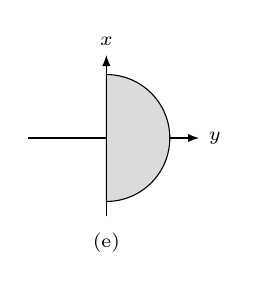
\begin{tikzpicture}[scale=0.62]
  \draw[-{Latex[length=4pt]}] (-1.6,0) -- (1.9,0) node[right,font=\scriptsize]{$y$};
  \draw[-{Latex[length=4pt]}] (0,-1.6) -- (0,1.7) node[above,font=\scriptsize]{$x$};
  \fill[black!14] (0,-1.3) arc (-90:90:1.3) -- cycle;
  \draw (0,-1.3) arc (-90:90:1.3) -- cycle;
  \node[font=\scriptsize] at (0,-2.15) {(e)};
\end{tikzpicture}}\hfil

\vspace{2pt}
\nota{Figura esquemática (redibujada de un escaneo). Las opciones (a)--(d) muestran el mismo tipo de sólido (casquete de paraboloide sobre un cono) cambiando la proyección sobre el plano $xy$ y la inclinación; (e) es una región plana. El sólido descrito por la integral es la porción con $x\geq 0$ de la región acotada abajo por el cono $z=\sqrt{x^2+y^2}$ y arriba por el paraboloide $z=2-x^2-y^2$ (se cortan en $x^2+y^2=1$); su proyección sobre el plano $xy$ es el semidisco $x^2+y^2\leq 1$, $x\geq 0$ --- opción \textbf{(d)}.}

\item (5\,\%) Al cambiar la integral triple dada a coordenadas cilíndricas se obtiene:
\begin{opciones}
\item $\displaystyle\int_0^{\pi} \int_0^1 \int_{r}^{2-r^2} f(r\cos\theta, r\operatorname{sen}\theta, z)\,r\,dz\,dr\,d\theta$
\item $\displaystyle\int_0^{\pi/2} \int_0^1 \int_{r}^{2-r^2} f(r\cos\theta, r\operatorname{sen}\theta, z)\,r\,dz\,dr\,d\theta$
\item $\displaystyle\int_{-\pi/2}^{\pi/2} \int_0^1 \int_{r}^{2-r^2} f(r\cos\theta, r\operatorname{sen}\theta, z)\,r\,dz\,dr\,d\theta$
\item $\displaystyle\int_0^1 \int_0^{\pi/2} \int_{2-r^2}^{r} f(r\cos\theta, r\operatorname{sen}\theta, z)\,r\,dz\,d\theta\,dr$
\item Ninguna de las anteriores.
\end{opciones}

\item (5\,\%) El valor de $\displaystyle\int_0^{\pi} \int_{-\sqrt{\pi^2-y^2}}^{\sqrt{\pi^2-y^2}} dx\,dy$ es:
\begin{opciones}
\item $\pi^2/2$
\item $\pi^2$
\item $\pi^3$
\item $\pi^3/2$
\item Ninguna de las anteriores.
\end{opciones}

\item (5\,\%) Considere la siguiente igualdad
\[
\iint_D f(x,y)\,dA = \lim_{m\to\infty} \lim_{n\to\infty} \sum_{i=1}^m \sum_{j=1}^n \frac{i\,j}{m^2 n^2}.
\]
Usando la esquina superior derecha de cada subrectángulo, la función $f$ y la región de integración $D$ que hacen válida dicha igualdad son:
\begin{opciones}
\item $f(x,y) = \dfrac{1}{x^2 y^2}$ \quad y \quad $D = \{(x,y) \in \mathbb{R}^2 : 0 \leq x \leq 2,\ 0 \leq y \leq 2\}$.
\item $f(x,y) = \dfrac{1}{xy}$ \quad y \quad $D = \{(x,y) \in \mathbb{R}^2 : 0 \leq x \leq 1,\ 0 \leq y \leq 1\}$.
\item $f(x,y) = xy$ \quad y \quad $D = \{(x,y) \in \mathbb{R}^2 : 0 \leq x \leq 1,\ 0 \leq y \leq 1\}$.
\item $f(x,y) = x^2 y^2$ \quad y \quad $D = \{(x,y) \in \mathbb{R}^2 : 0 \leq x \leq 2,\ 0 \leq y \leq 2\}$.
\item Ninguna de las anteriores.
\end{opciones}
\end{enumerate}

\item{} (25\,\%) Sea $\delta(x,y) = e^{-xy}$ la densidad en cada punto $(x,y)$ de la placa $R = \{(x,y) \in \mathbb{R}^2 : x^2 + 4y^2 \leq 1\}$.
\begin{enumerate}[label=(\alph*)]
\item (10\,\%) Sabiendo que las únicas soluciones del sistema
\[
\vec\nabla \delta(x,y) = \lambda\,\vec\nabla(x^2 + 4y^2), \qquad x^2 + 4y^2 = 1
\]
son
\[
(x,y,\lambda) = \left(\tfrac{1}{\sqrt2}, \tfrac{1}{\sqrt8}, -\tfrac{e^{-1/4}}{4}\right),\
\left(-\tfrac{1}{\sqrt2}, -\tfrac{1}{\sqrt8}, -\tfrac{e^{-1/4}}{4}\right),\
\left(-\tfrac{1}{\sqrt2}, \tfrac{1}{\sqrt8}, \tfrac{e^{1/4}}{4}\right)
\]
y $\left(\tfrac{1}{\sqrt2}, -\tfrac{1}{\sqrt8}, \tfrac{e^{1/4}}{4}\right)$, halle los valores máximo y mínimo absolutos de $\delta$ en $R$ (justifique completamente).
\item (15\,\%) Estime el valor de la masa $m(R)$ de $R$, es decir, halle constantes positivas $A$ y $B$ tales que $A \leq m(R) \leq B$.
\end{enumerate}

\item{} (25\,\%) Sea $D$ la región del primer cuadrante acotada por las curvas $xy = 1$, $xy = 3$, $x^2 - y^2 = 1$ y $x^2 - y^2 = 4$. Calcule
\[
\iint_D (x^2 + y^2)\operatorname{sen}(x^2 - y^2)\,dA.
\]
Dibuje claramente la región de integración de toda integral que escriba.

\item{} (25\,\%) Halle el volumen del sólido en el primer octante limitado por la esfera $x^2 + y^2 + z^2 = 1$, el cono $3(x^2 + y^2) = z^2$, el plano $y = \sqrt3\,x$, el plano $x = 0$, y el cono $x^2 + y^2 = z^2$.
\end{enumerate}

\examfooter

\end{document}
